\chapter{Descrierea Aplicației TickLy}
\label{sec:descriere-aplicatie}

Sistemul TickLy este o platformă de tip Help Desk concepută pentru gestionarea incidentelor și solicitărilor de suport. Aplicația oferă funcționalități de bază pentru managementul fluxului de lucru și analiză avansată a datelor prin module de raportare.

\section{Funcționalități Principale}
Aplicația permite realizarea următoarelor operațiuni:
\begin{itemize}
    \item \textbf{Management Tichete (CRU):} Utilizatorii pot crea, vizualiza si actualiza. Fiecare tichet include detalii despre prioritate, status, departament și subiectul vizat.
    \item \textbf{Comunicare și Colaborare:} Sistem de comentarii integrat pentru clienți și agenți, permițând monitorizarea istoricului conversației și jurnalizarea acțiunilor de audit în \textit{Ticket History}.
    \item \textbf{Modul de Raportare OLAP:} Dashboard integrat care se foloseste date din OLAP prin \textit{Materialized Views} pentru a vizualiza performanța operațională.
\end{itemize}

\begin{figure}[H]
    \centering
    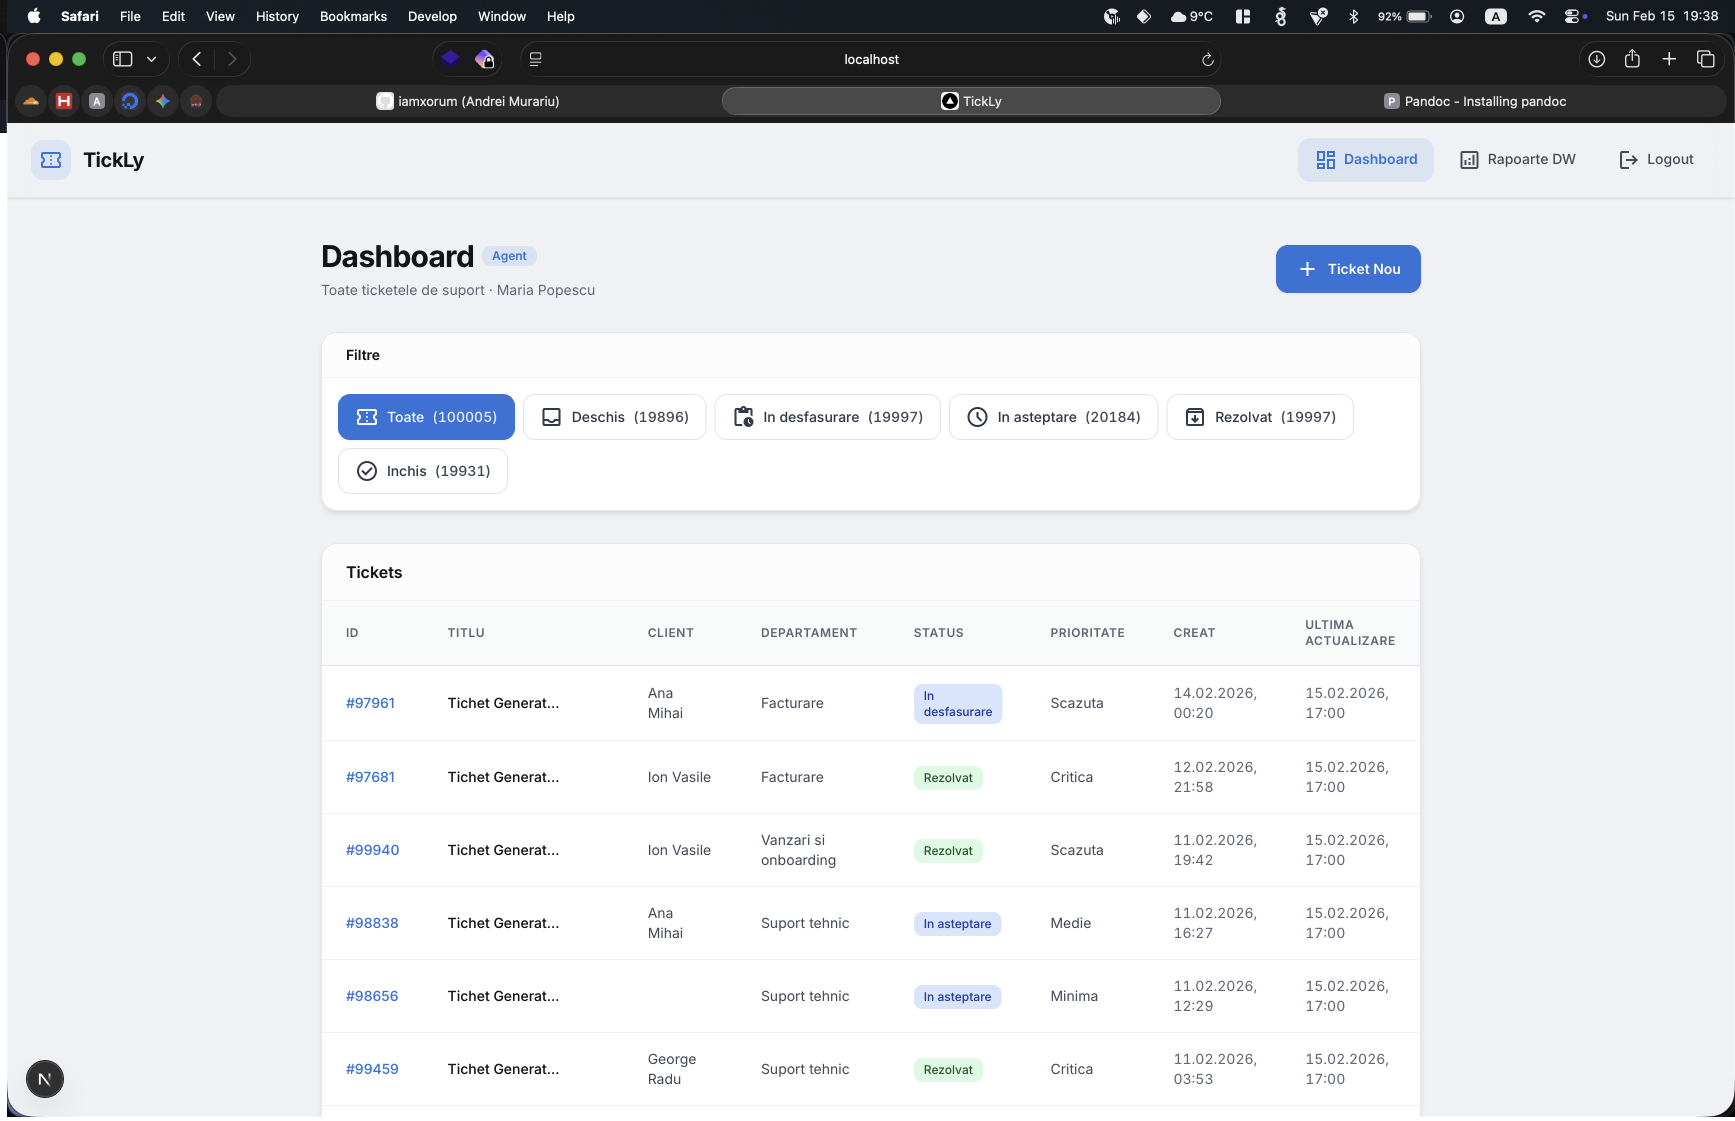
\includegraphics[width=0.6\textwidth]{./assets/app/dashboard.png}
    \caption{Dashboard}
    \label{fig:dashboard}
\end{figure}

\begin{figure}[H]
    \centering
    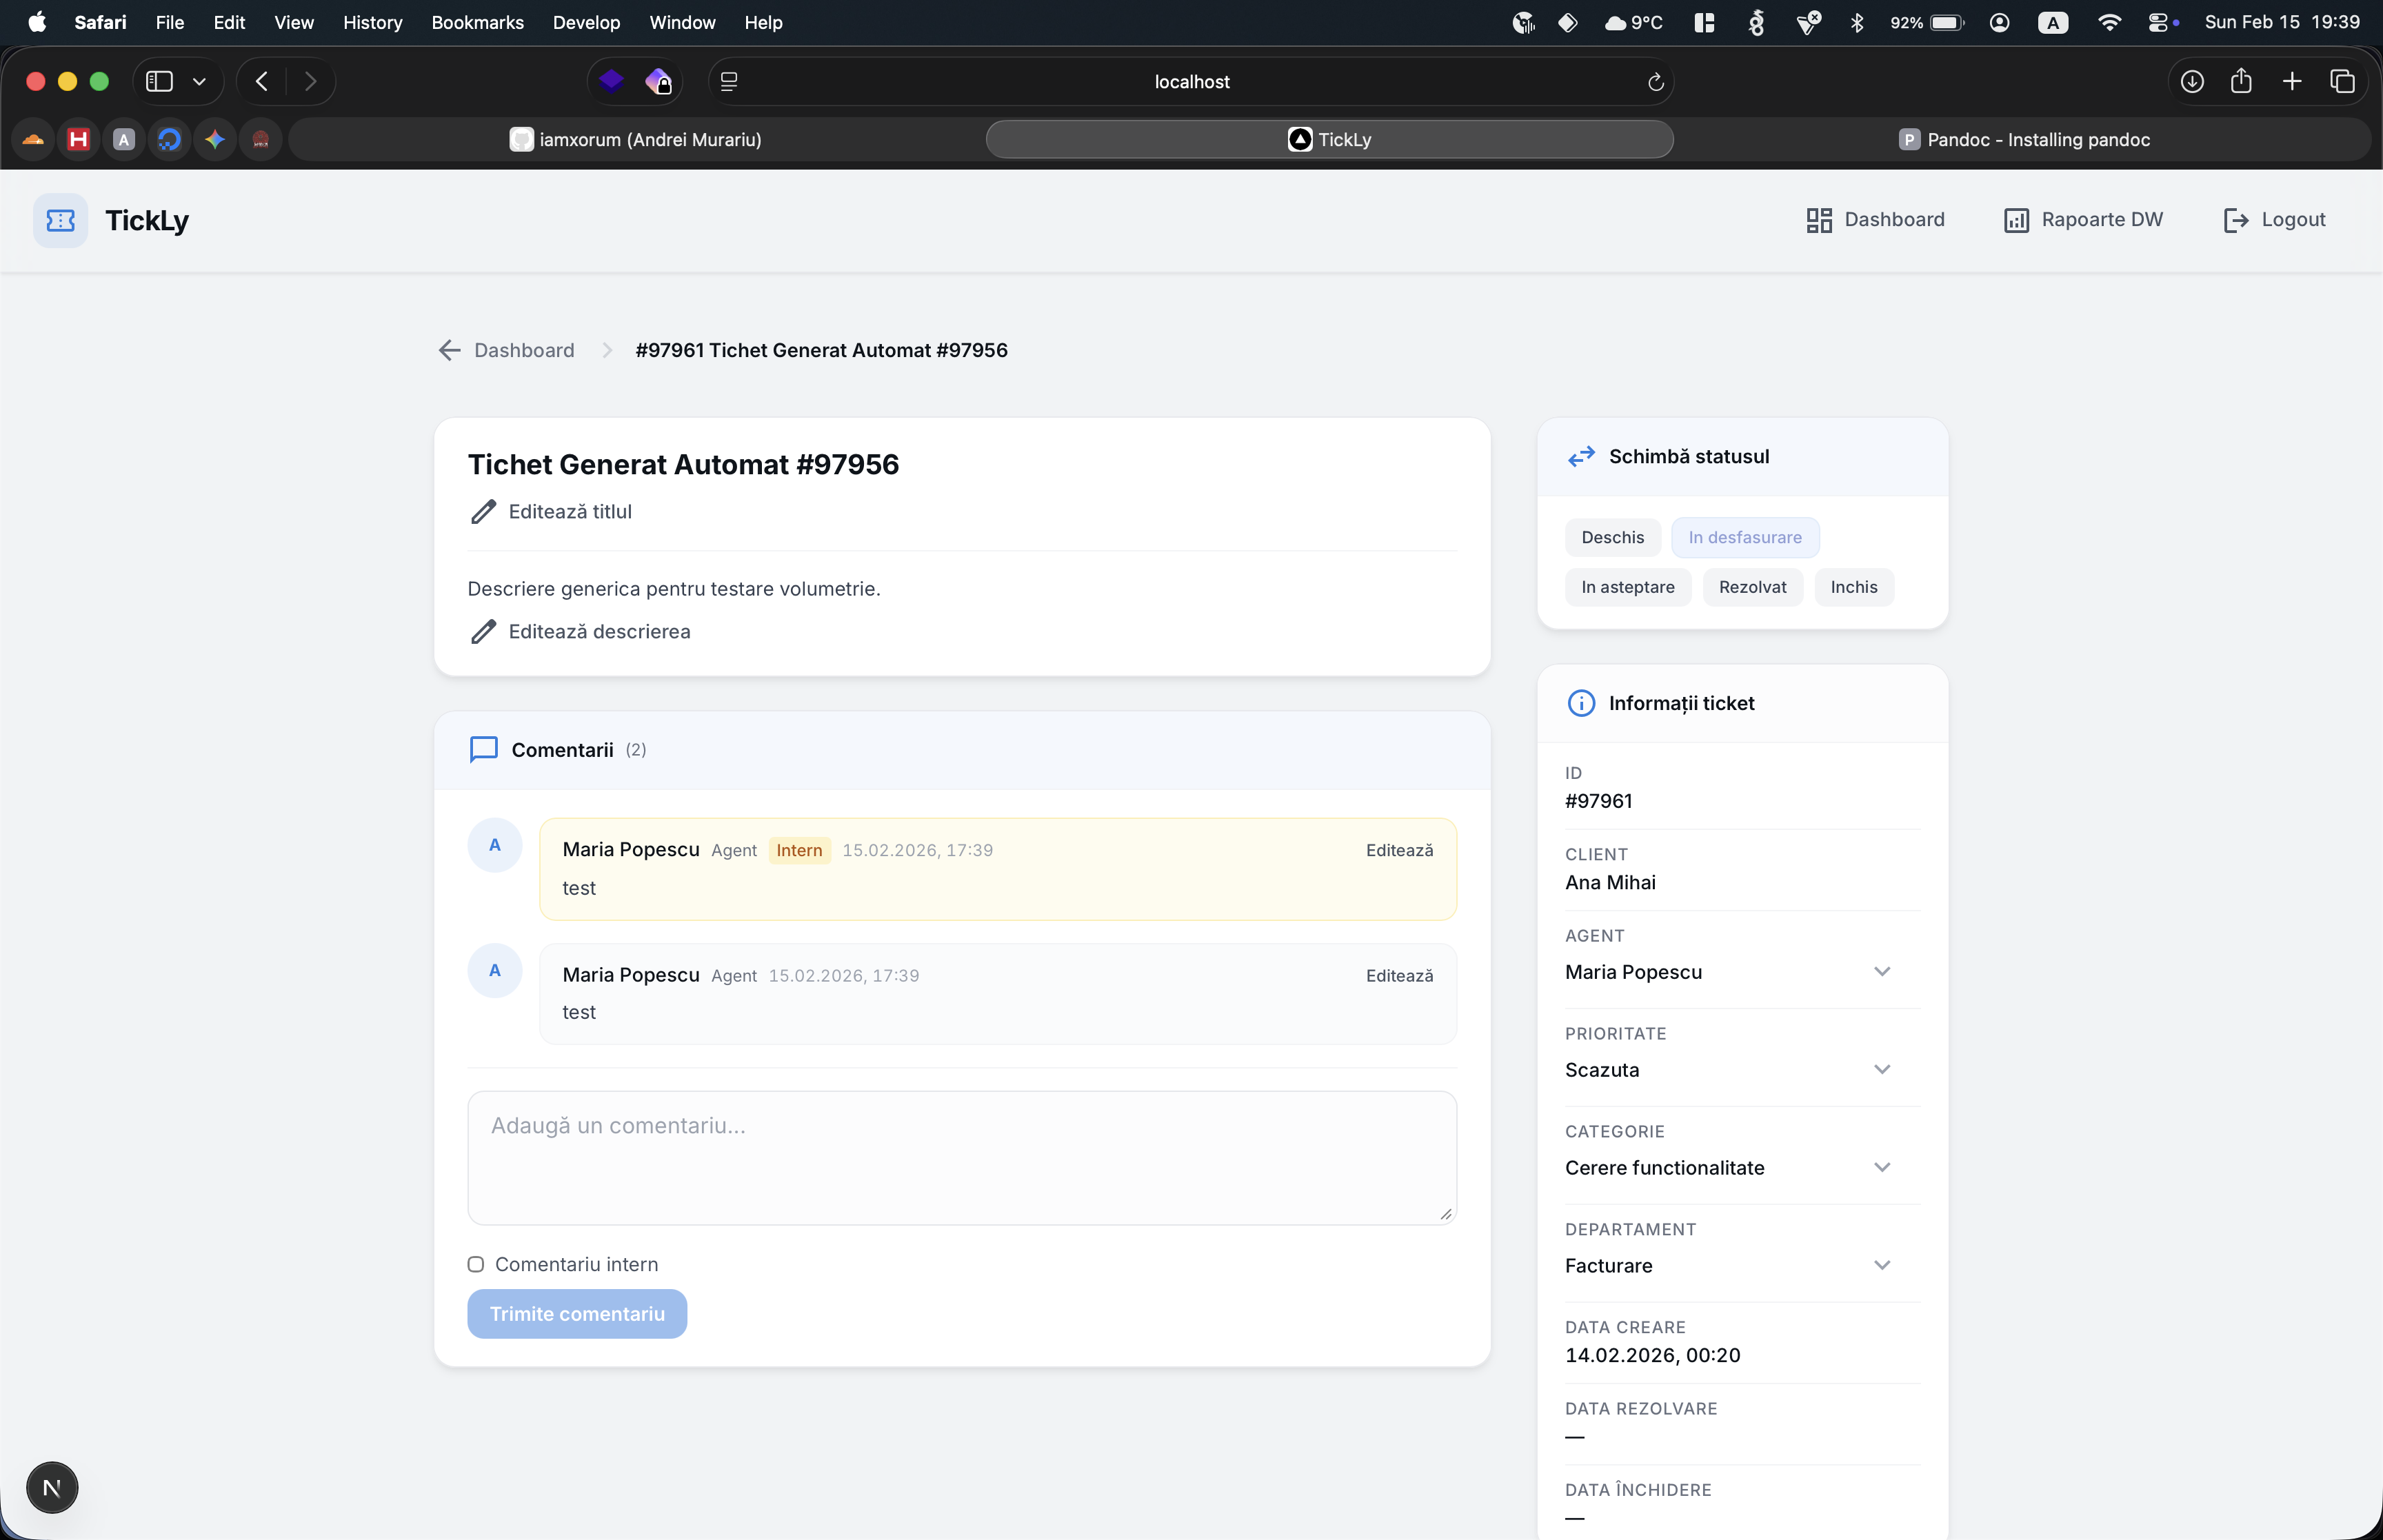
\includegraphics[width=0.6\textwidth]{./assets/app/ticket.png}
    \caption{Ticket}
    \label{fig:tkt}
\end{figure}

\begin{figure}[H]
    \centering
    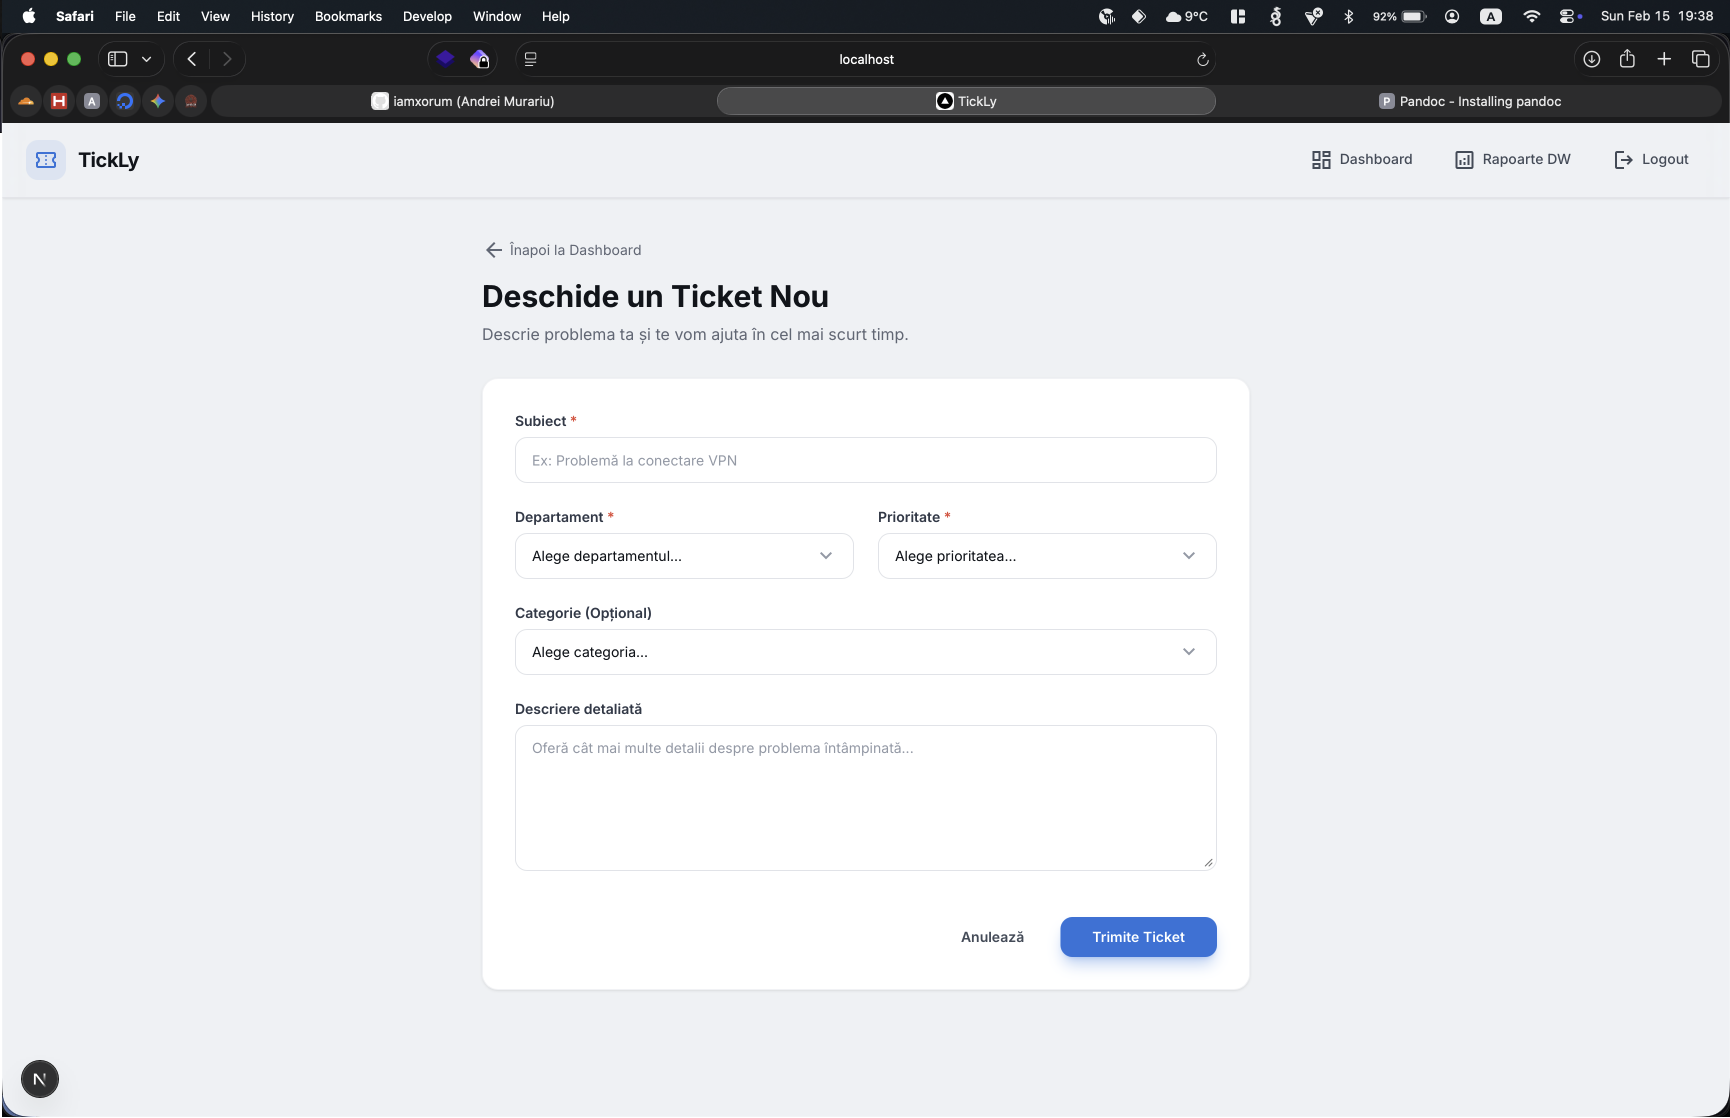
\includegraphics[width=0.6\textwidth]{./assets/app/new_ticket.png}
    \caption{New ticket}
    \label{fig:new_tkt}
\end{figure}

\begin{figure}[H]
    \centering
    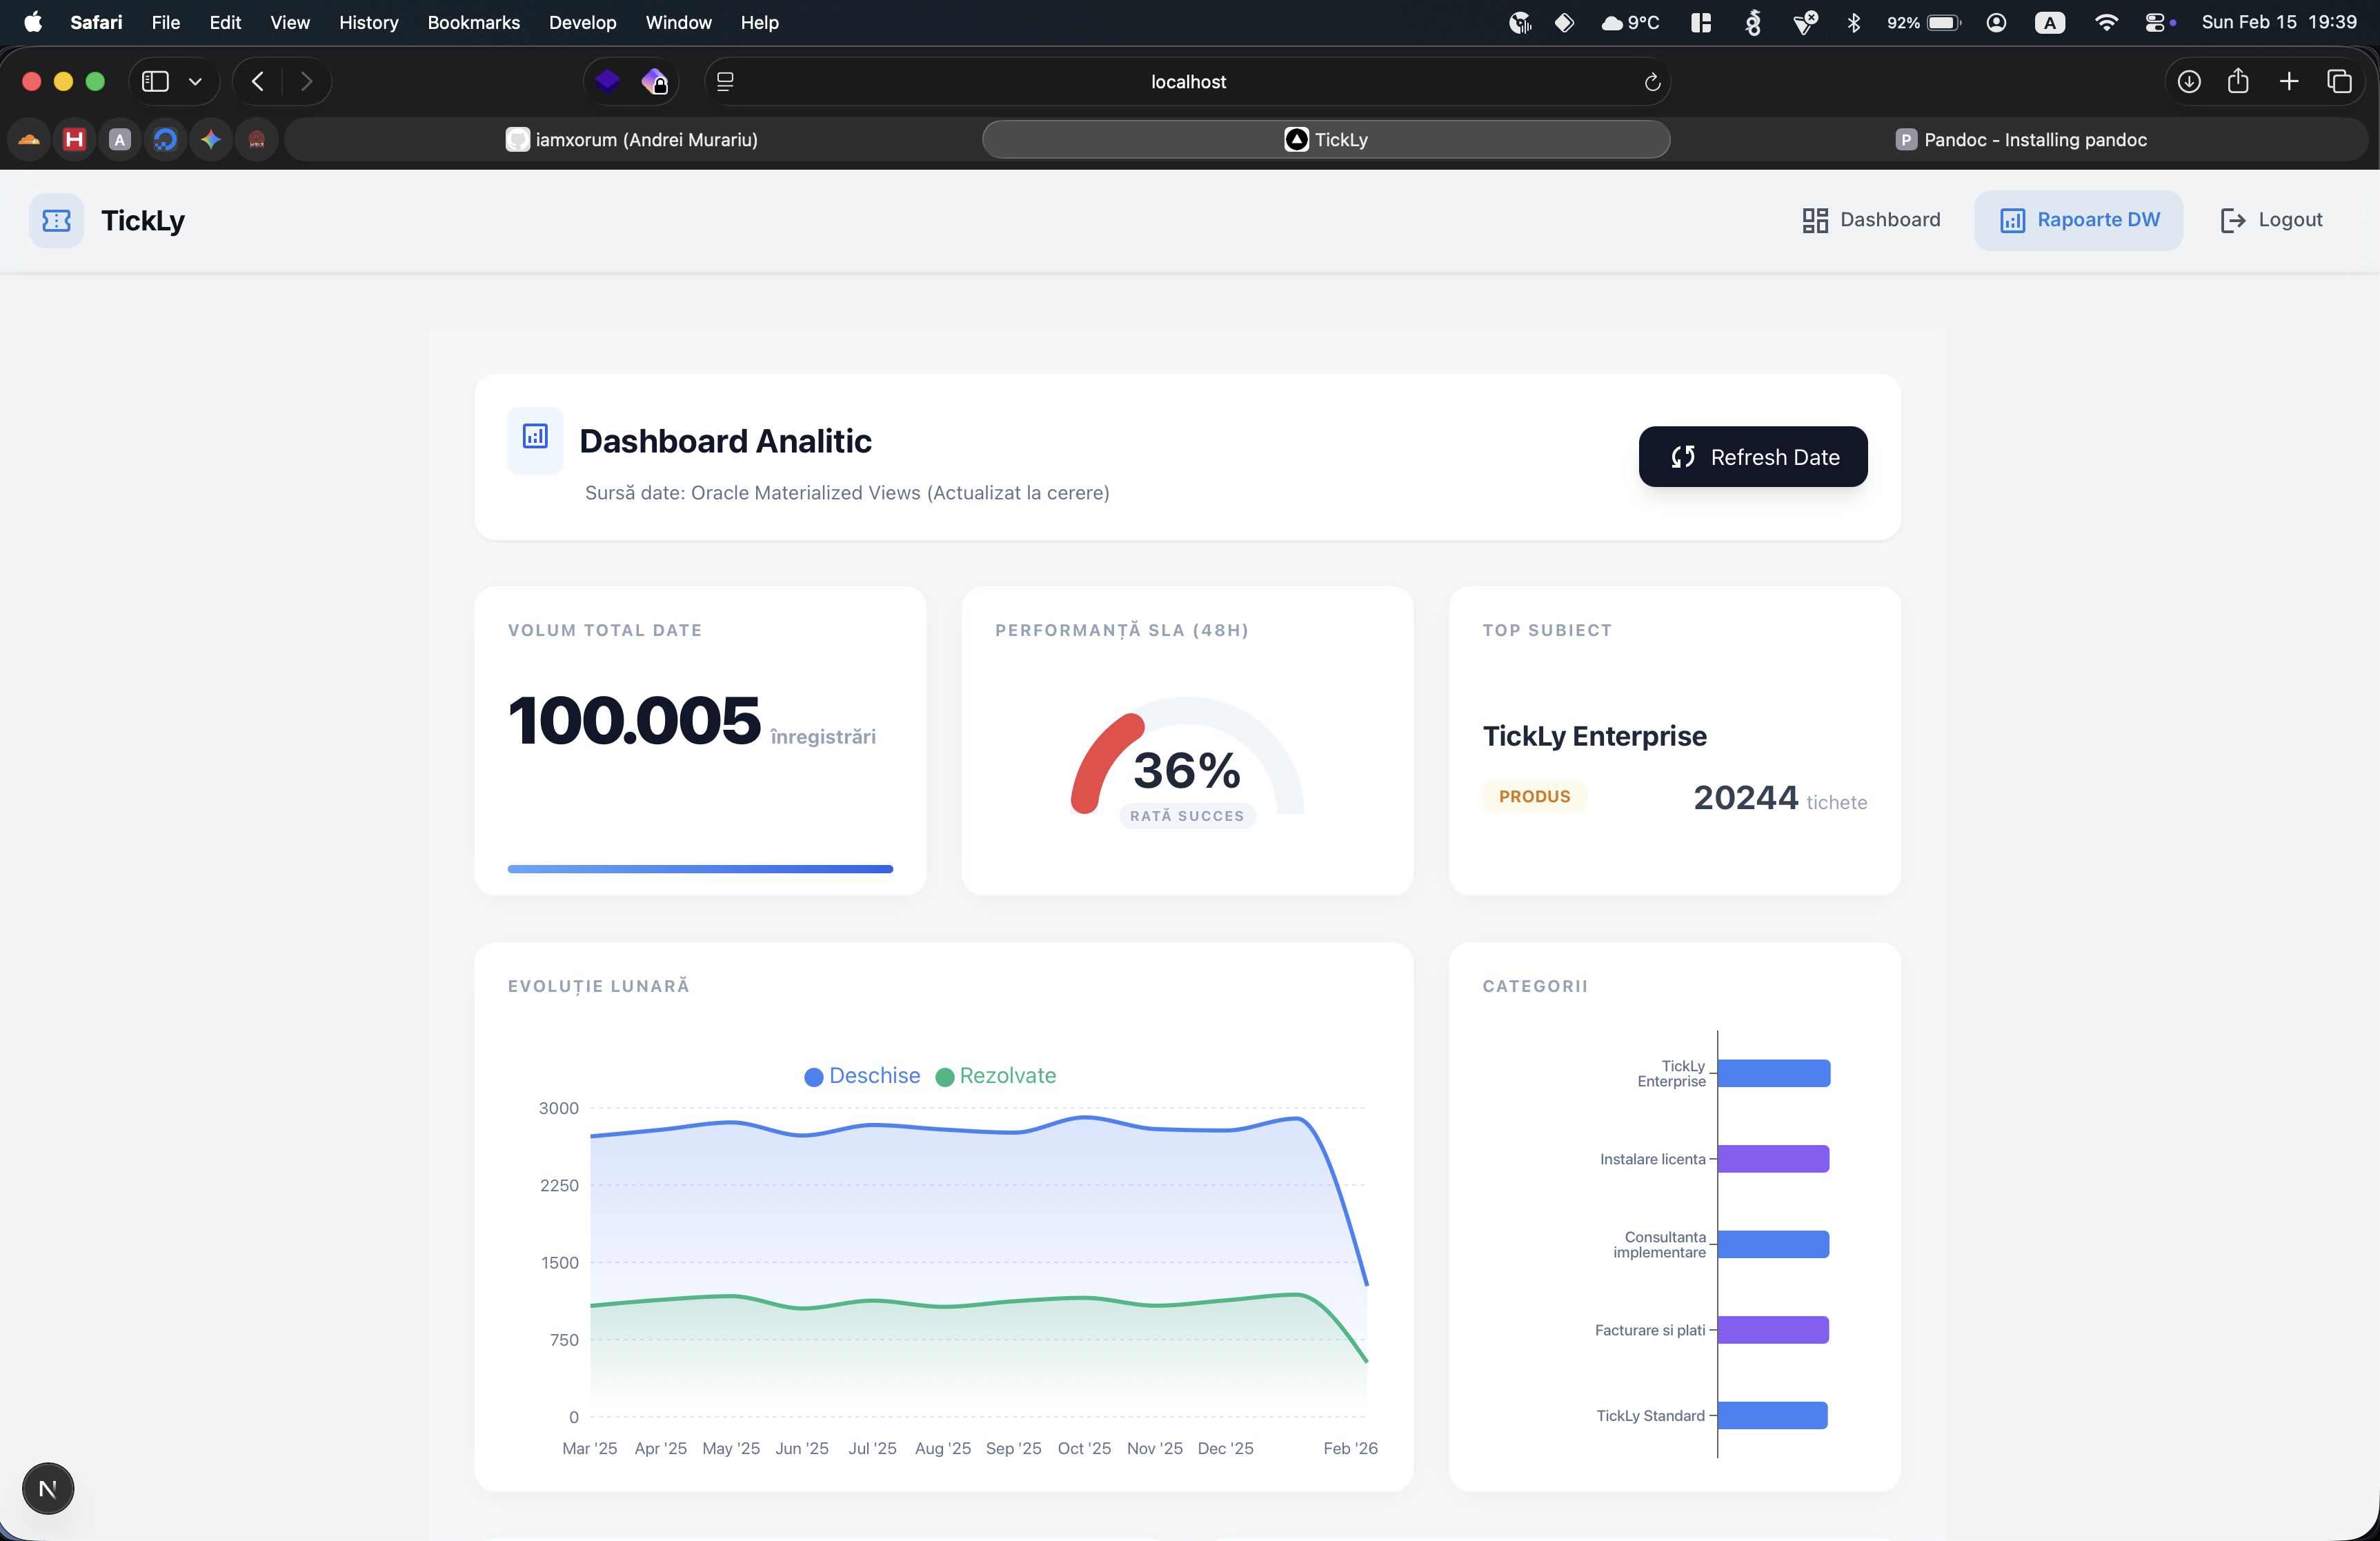
\includegraphics[width=0.6\textwidth]{./assets/app/reports.png}
    \caption{Reports}
    \label{fig:reports}
\end{figure}